\chapter{Cải thiện chất lượng phản hồi của Chatbot sử dụng RAG và đồ thị tri thức}
\label{chapter:proposed_method}


Hiện nay, với với khả năng mạnh mẽ của LLM, Chatbot đã trở thành một công cụ hữu ích trong việc hỗ trợ người dùng truy cập thông tin, giải đáp thắc mắc. Tuy nhiên, mặc dù có khả năng học và tự cải thiện, Chatbot vẫn còn một số hạn chế trong việc cập nhật thông tin kịp thời cũng như đôi lúc vẫn còn hiện tượng ảo giác với tác vụ Q\&A trong miền tri thức với tài liệu đã được chuẩn hóa. Trong chương này, tôi đề xuất một phương pháp kết hợp giữa \gls{rag} và đồ thị tri thức để cải thiện khả năng hỗ trợ hỏi đáp của Chatbot từ tài liệu. Phương pháp này sẽ giúp cải thiện khả năng truy xuất thông tin, suy luận thông qua việc kết hợp giữa việc mở rộng chuỗi logic dựa trên các liên kết trong \gls{kg} với thông tin ngữ cảnh liên kết với các thực thể liên quan bằng cách thực hiện lặp đi lặp lại việc truy xuất ngữ cảnh dựa tri thức và sử dụng ngữ cảnh tăng cường truy xuất đồ thị. Từ đó tích hợp và sử dụng hiệu quả hơn kiến thức bên ngoài từ các dạng cấu trúc khác nhau.


Nội dung chính của phương pháp đề xuất gồm có 2 phần, đầu tiên là phần \ref{section:database_construction_method} thảo luận về phương pháp xây dựng đồ thị tri thức, cơ sở dữ liệu từ những tài liệu được cung cấp. Tiếp đó phần \ref{section:rag_integrated_knowledge_graph} mô tả cốt lõi khả năng của một Chatbot là phương pháp \gls{rag} tích hợp truy xuất, suy luận đồ thị tri thức với truy xuất cơ sở dữ liệu vector để nâng cao khả năng của mô hình ngôn ngữ lớn (LLMs). Phương pháp đề xuất kết hợp việc mở rộng chuỗi logic dựa trên các liên kết trong \gls{kg} với thông tin ngữ cảnh liên kết với các thực thể liên quan bằng cách thực hiện lặp đi lặp lại việc truy xuất ngữ cảnh dựa tri thức và sử dụng ngữ cảnh tăng cường truy xuất đồ thị. từ đó tích hợp và sử dụng hiệu quả hơn kiến thức bên ngoài từ các dạng cấu trúc khác nhau.


\section{Các thuật ngữ cơ bản}
\label{section:terminology}
Trước khi đi vào chi tiết phương pháp đề xuất, tôi xin trình bày một số thuật ngữ cơ bản mà sẽ được sử dụng trong phần này:
\begin{itemize}
    \item \textbf{Knowledge Graph - Đồ thị tri thức} chứa đựng, biểu diễn các kiến thức trong thế giới thực dưới dạng tập các bộ ba: \[
              G = \{(e, r, e') | e, e' \in \mathcal{E}, r \in \mathcal{R}\},
          \]
          Trong đó $\mathcal{E}$ và $\mathcal{R}$ tương ứng biểu thị cho tập thực thể và quan hệ.


    \item \textbf{Relation Path - Đường dẫn quan hệ} là một chuỗi các quan hệ $z = \{r_1, r_2, \dots, r_l\}$ trong đó $r_i \in \mathcal{R}$ biểu thị cho mối quan hệ thứ $i$ trong đường dẫn có độ dài là $l$.
    \item \textbf{Reasoning Path - Đường dẫn suy luận} là các thể hiện của đường dẫn quan hệ $z$ trong \gls{kg}s: \[
              p_{\{z\}} = e_0 \xrightarrow{r_1} e_1 \xrightarrow{r_2} \cdots \xrightarrow{r_l} e_l,
          \] trong đó $e_i \in \mathcal{E}$ biểu thị cho thực thể thứ $i$ và $r_i$ biểu thị cho mối quan hệ thứ $i$ trong đường dẫn suy luận $p$.
    \item \textbf{Prompt - lời nhắc} được sử dụng trong khóa luận về cơ bản là đầu vào được cung cấp cho \gls{llm}s để tạo ra các đầu ra có định hướng. Mục đích của một prompt là chỉ định rõ \gls{llm}s cần tạo ra gì để giúp chúng có thể hiểu ngữ cảnh và thực hiện các tác vụ cụ thể rồi đưa ra đầu ra mong muốn.
    \item \textbf{Tài liệu chuẩn hóa} là các tài liệu được xây dựng một cách có cấu trúc, với các chỉ mục được phân chia một cách rõ ràng và hợp lý. Từ đó chia nội dung của tài liệu thành các đoạn nhỏ có nội dung cụ thể về một ngữ cảnh và các mục nhỏ trong cùng một mục lớn hơn sẽ có sự liên quan về ngữ cảnh.
    \item \textbf{Ontology} là một mô hình học thức học được sử dụng để biểu diễn kiến thức trong một lĩnh vực cụ thể. Ontology thường bao gồm các thực thể, mối quan hệ, hành động, sự kiện, và các khái niệm khác trong một lĩnh vực cụ thể.
\end{itemize}


\section{Xây dựng đồ thị tri thức, cơ sở dữ liệu từ những tài liệu chuẩn hóa}
\label{section:database_construction_method}
Việc lưu trữ các tài liệu cũng như tri thức từ các tài liệu dưới dạng đồ thị tri thức (Knowledge Graph - \gls{kg}) và các đoạn văn là một phần quan trọng trong phương pháp được đề xuất. Trong phần này, tôi sẽ trình bày chi tiết phương pháp xây dựng, lưu trữ đồ thị tri thức và cây tài liệu từ những tài liệu đó. Kết quả của quá trình này được minh họa trong hình \ref{fig:kg_construction}.


\begin{figure}
    \centering
    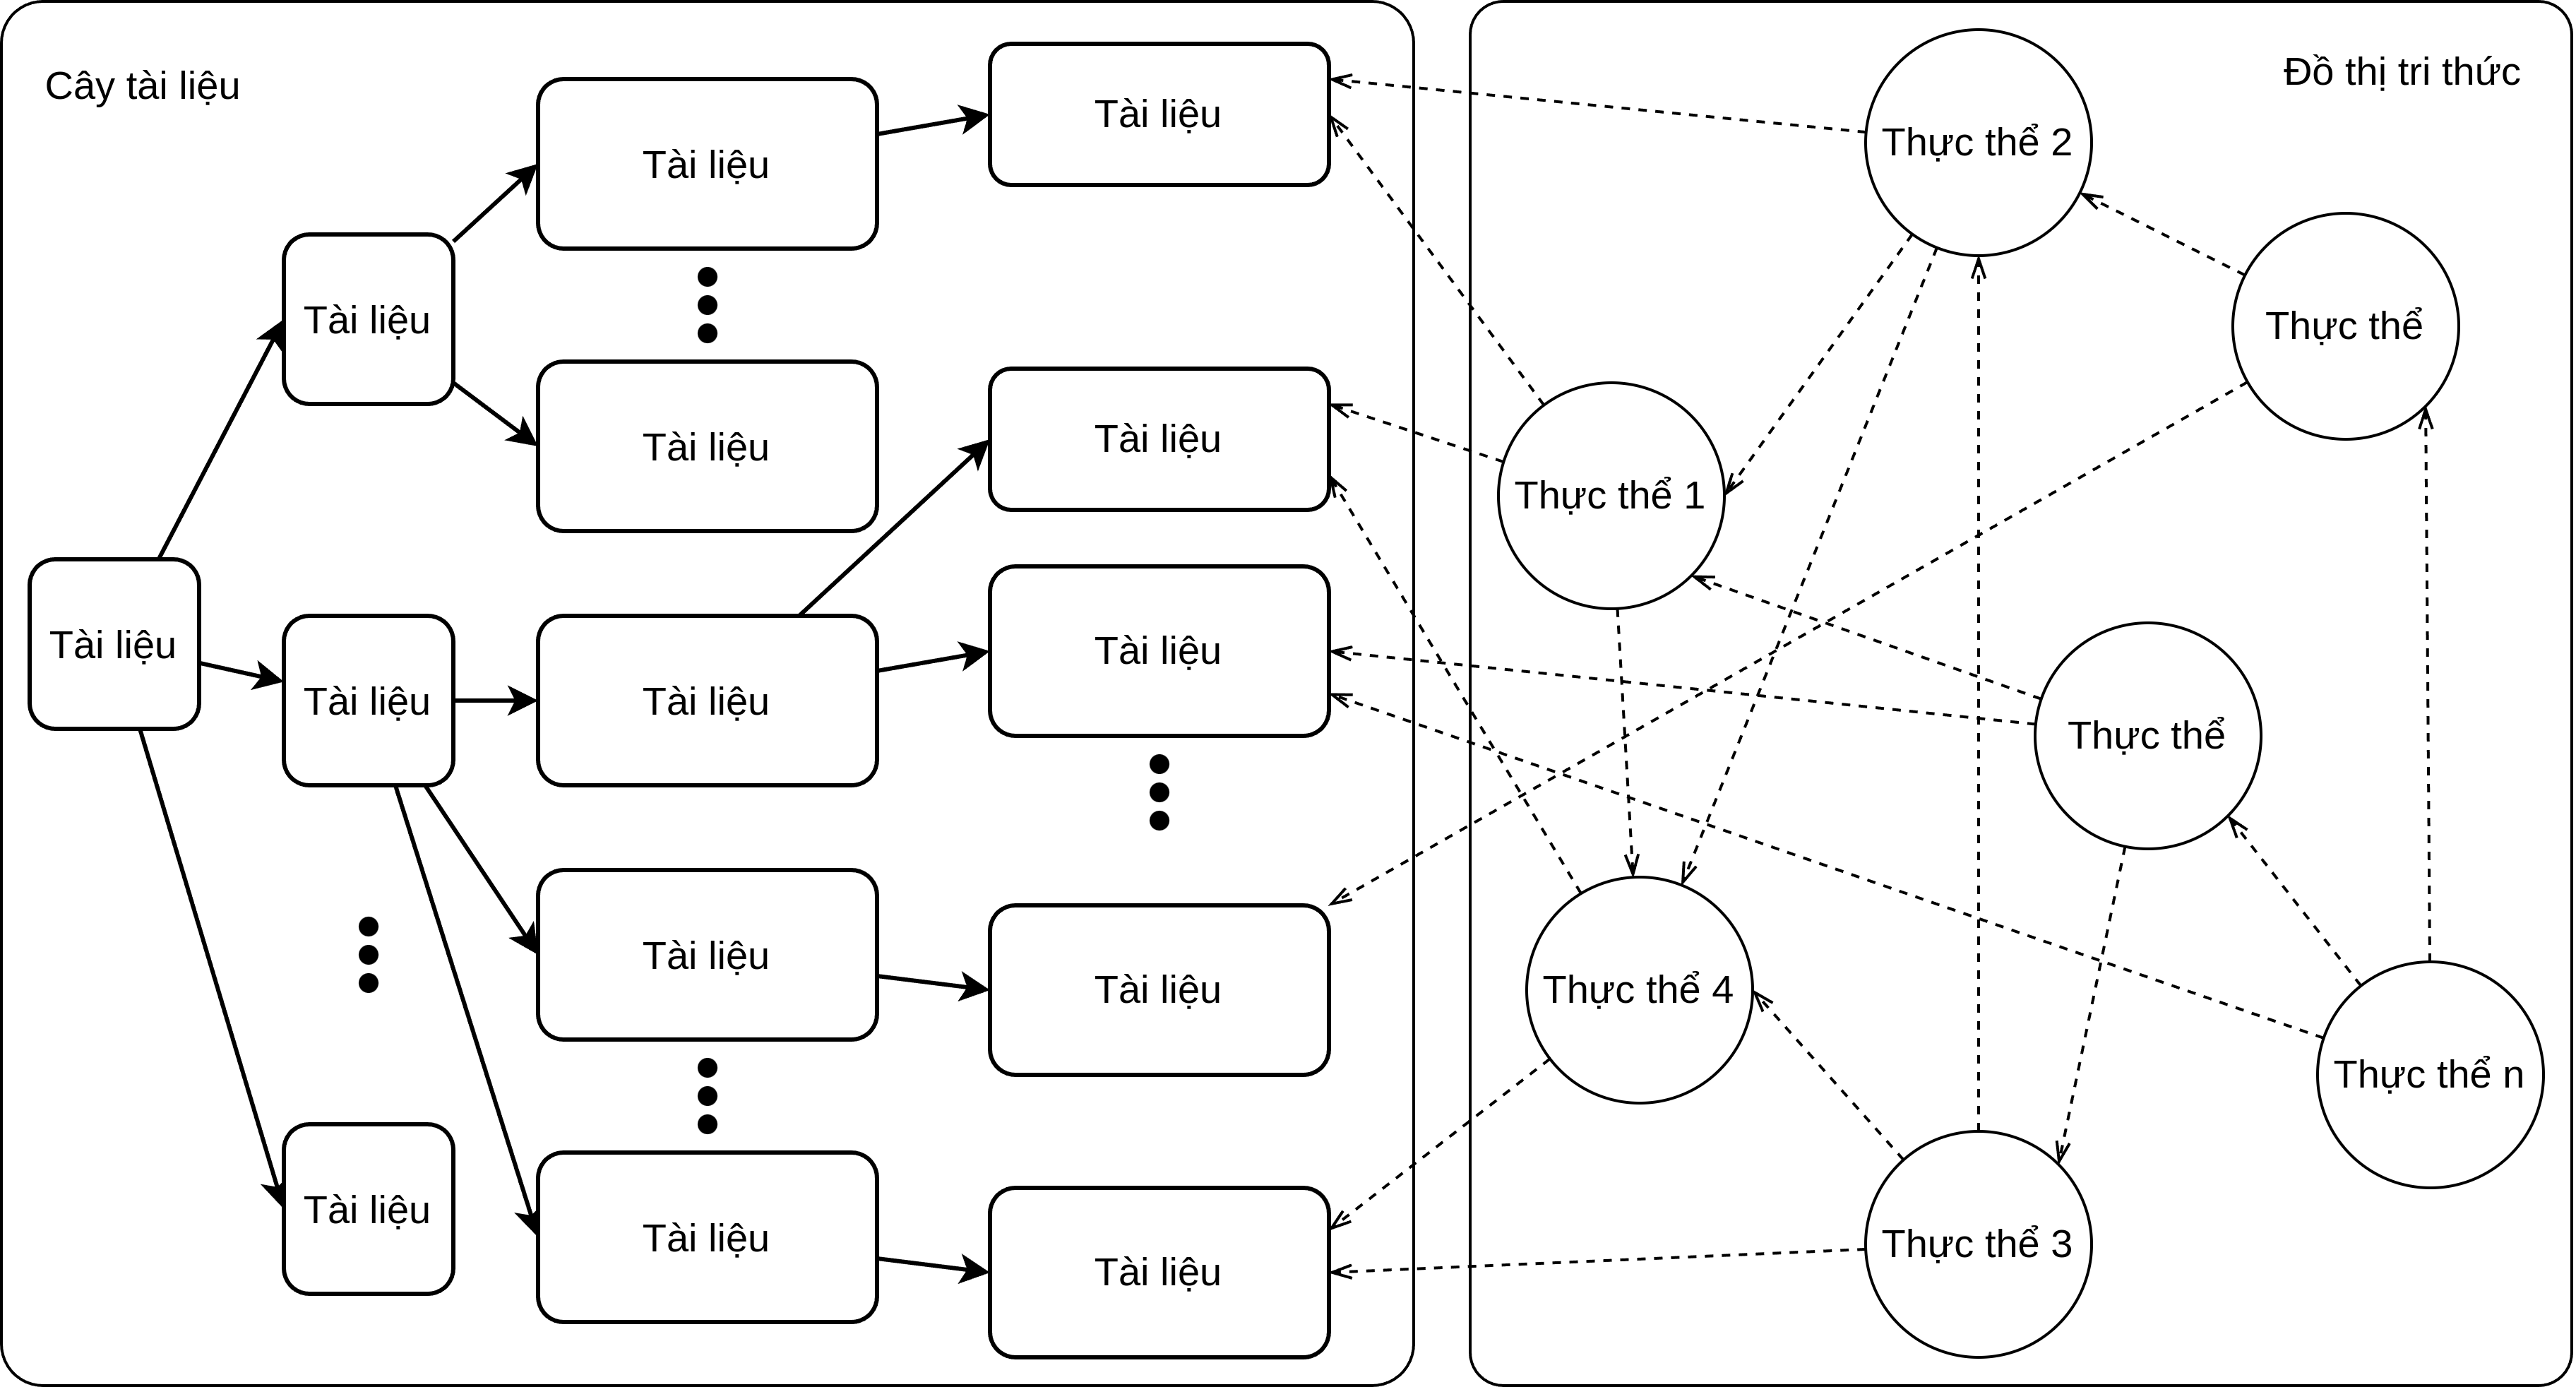
\includegraphics[width=1\textwidth]{Chapter3/Fig/database_construction.png}
    \caption{Minh họa xây dựng đồ thị tri thức, cây tài liệu từ tài liệu chuẩn hóa}
    \label{fig:kg_construction}
\end{figure}
\subsection{Xây dựng cây tài liệu từ tài liệu chuẩn hóa}
\label{subsection:document_tree_construction}
Trong phạm vi là các tài liệu chuẩn hóa, thì các tài liệu này đều sẽ là dạng văn bản bán cấu trúc với các tiêu đề, đoạn văn, câu, từ, ... Để tận dụng được cấu trúc của các tài liệu này, một cây tài liệu sẽ được xây dựng từ các tài liệu. Cây tài liệu này sẽ được xây dựng dựa trên mục lục của tài liệu. Mỗi nút trong cây tài liệu sẽ biểu diễn một phần của tài liệu, từ đó giúp cho việc truy xuất thông tin từ tài liệu trở nên dễ dàng hơn. Với việc xây dựng cây tài liệu, việc truy xuất thông tin từ tài liệu sẽ trở nên dễ dàng hơn cũng như có thể phản ảnh được mối liên quan giữa các tài liệu với nhau thông qua khoảng cách giữa các nút trong cây tài liệu. Càng gần nhau thì mối liên quan về ngữ cảnh giữa các tài liệu càng cao.




\subsection{Xây dựng đồ thị tri thức từ tài liệu chuẩn hóa}
\label{subsection:knowledge_graph_construction_from_document}
Một đồ thị tri thức (KG) là một biểu diễn có cấu trúc của các thực thể trong thế giới thực, các thuộc tính của chúng và mối quan hệ giữa chúng. Một \gls{kg} được biểu diễn dưới dạng một tập hợp các bộ ba có hướng \((\text{thực thể}, \text{mối quan hệ}, \text{thực thể})\).  Một bộ ba đồ thị là một đơn vị thông tin cơ bản trong một \gls{kg}, bao gồm một chủ ngữ, một vị ngữ và một tân ngữ.
Với mỗi miền tri thức cụ thể ứng với tài liệu chuẩn hóa, một Ontology tương ứng sẽ được xây dựng nhằm tối ưu hóa việc trích xuất tri thức từ tài liệu. Dựa trên cây tài liệu và Ontology đã xây dựng, một \gls{kg} sẽ được xây dựng và liên kết với tài liệu tương ứng. Quá trình này sẽ bao gồm hai phần chính là trích xuất tri thức và cải thiện tri thức.


\paragraph{Trích xuất tri thức:}
\label{paragraph:extract_knowledge}
Mục tiêu của bước này đến việc chuyển đổi thông tin, tri thức từ dữ liệu không có cấu trúc như văn bản thành một \gls{kg} có cấu trúc có thể được truy vấn sau này. Quá trình này chủ yếu phụ thuộc vào việc trích xuất các bộ ba có định dạng là \(
\text{(thực thể)} \ - \ \left[\text{mối quan hệ}\right] \ \rightarrow \ \text{(thực thể)}
\). Để giúp cho các thực thể được trích xuất là những thực thể tổng quan và tránh những thông tin dư thừa, một Ontology sẽ được sử dụng để hướng dẫn quá trình trích xuất tri thức. Ontology sẽ được xây dựng dựa trên kiến thức về miền tri thức cụ thể, thông qua thực nghiệm kèm theo hướng dẫn từ các chuyên gia trong lĩnh vực.
Hỗ trợ điều này, phương pháp few-shot prompt được áp dụng vào một LLM, yêu cầu nó trích xuất càng nhiều bộ ba càng tốt từ các đoạn văn bản, đồng thời đưa các ví dụ về chuyển đổi văn bản thành bộ ba vào trong câu lệnh. Các tác vụ chính trong bước này sẽ bao gồm nhận dạng thực thể (ER), trích xuất mối quan thông qua sử dụng \gls{llm} với prompt tương ứng (được trình bày tại \ref{tab:ER_prompt}).


\paragraph{Cải thiện tri thức:}
\label{paragraph:improve_knowledge}
Bước này nhằm nâng cao chất lượng và độ hoàn thiện của \gls{kg} bằng cách loại bỏ các thông tin dư thừa và khắc phục những lỗ hổng trong dữ liệu đã trích xuất. Các nhiệm vụ chính trong bước này bao gồm hoàn thiện \gls{kg} và hợp nhất tri thức.
Kỹ thuật hoàn thiện \gls{kg} tìm ra các thực thể, mối quan hệ còn thiếu trong đồ thị bằng phương pháp dự đoán liên kết và xác định thực thể. Dự đoán liên kết dự đoán sự tồn tại và loại mối quan hệ giữa hai thực thể dựa trên cấu trúc và đặc điểm của đồ thị. Trong khi đó xác định thực thể khớp và hợp nhất các thực thể cùng biểu diễn một thực thể, khái niệm trong thế giới thực.
Quá trình hợp nhất tri thức kết hợp thông tin từ nhiều nguồn khác nhau để tạo ra một \gls{kg} hoàn chỉnh và thống nhất. Các nguồn thông tin này có thể bao gồm các \gls{kg} khác, dữ liệu từ các nguồn bên ngoài, ... Quá trình này bao gồm giải quyết xung đột và trùng lặp giữa các nguồn và tổng hợp hoặc điều hòa thông tin dựa trên các quy tắc, xác suất, hoặc sự tương đồng ngữ nghĩa.


Một chuỗi \gls{llm} được triển khai gồm 2 tầng để tinh chỉnh nội dung và trích xuất tri thức. Tầng thứ nhất sử dụng một \gls{llm} để tạo ra biểu diễn tóm tắt cho từng đoạn tài liệu. Quá trình tinh chỉnh này rất quan trọng vì nó chắt lọc thông tin cốt lõi đồng thời giữ nguyên ý nghĩa ban đầu và các mối quan hệ chính giữa các khái niệm. Điều này cung cấp một đầu vào tập trung hơn cho các bước xử lý tiếp theo, nâng cao hiệu quả và độ chính xác của quy trình trích xuất bộ ba. Tầng thứ hai là một \gls{llm} dành riêng cho việc trích xuất thực thể và xác định mối quan hệ. Tất cả các bước đều được thực hiện thông qua kỹ thuật gợi ý (prompt engineering) một cách cẩn thận.
\section{Mô hình RAG tích hợp truy xuất, suy luận đồ thị tri thức với truy xuất cơ sở dữ liệu vector}
\label{section:rag_integrated_knowledge_graph}
\begin{figure}
    \centering
    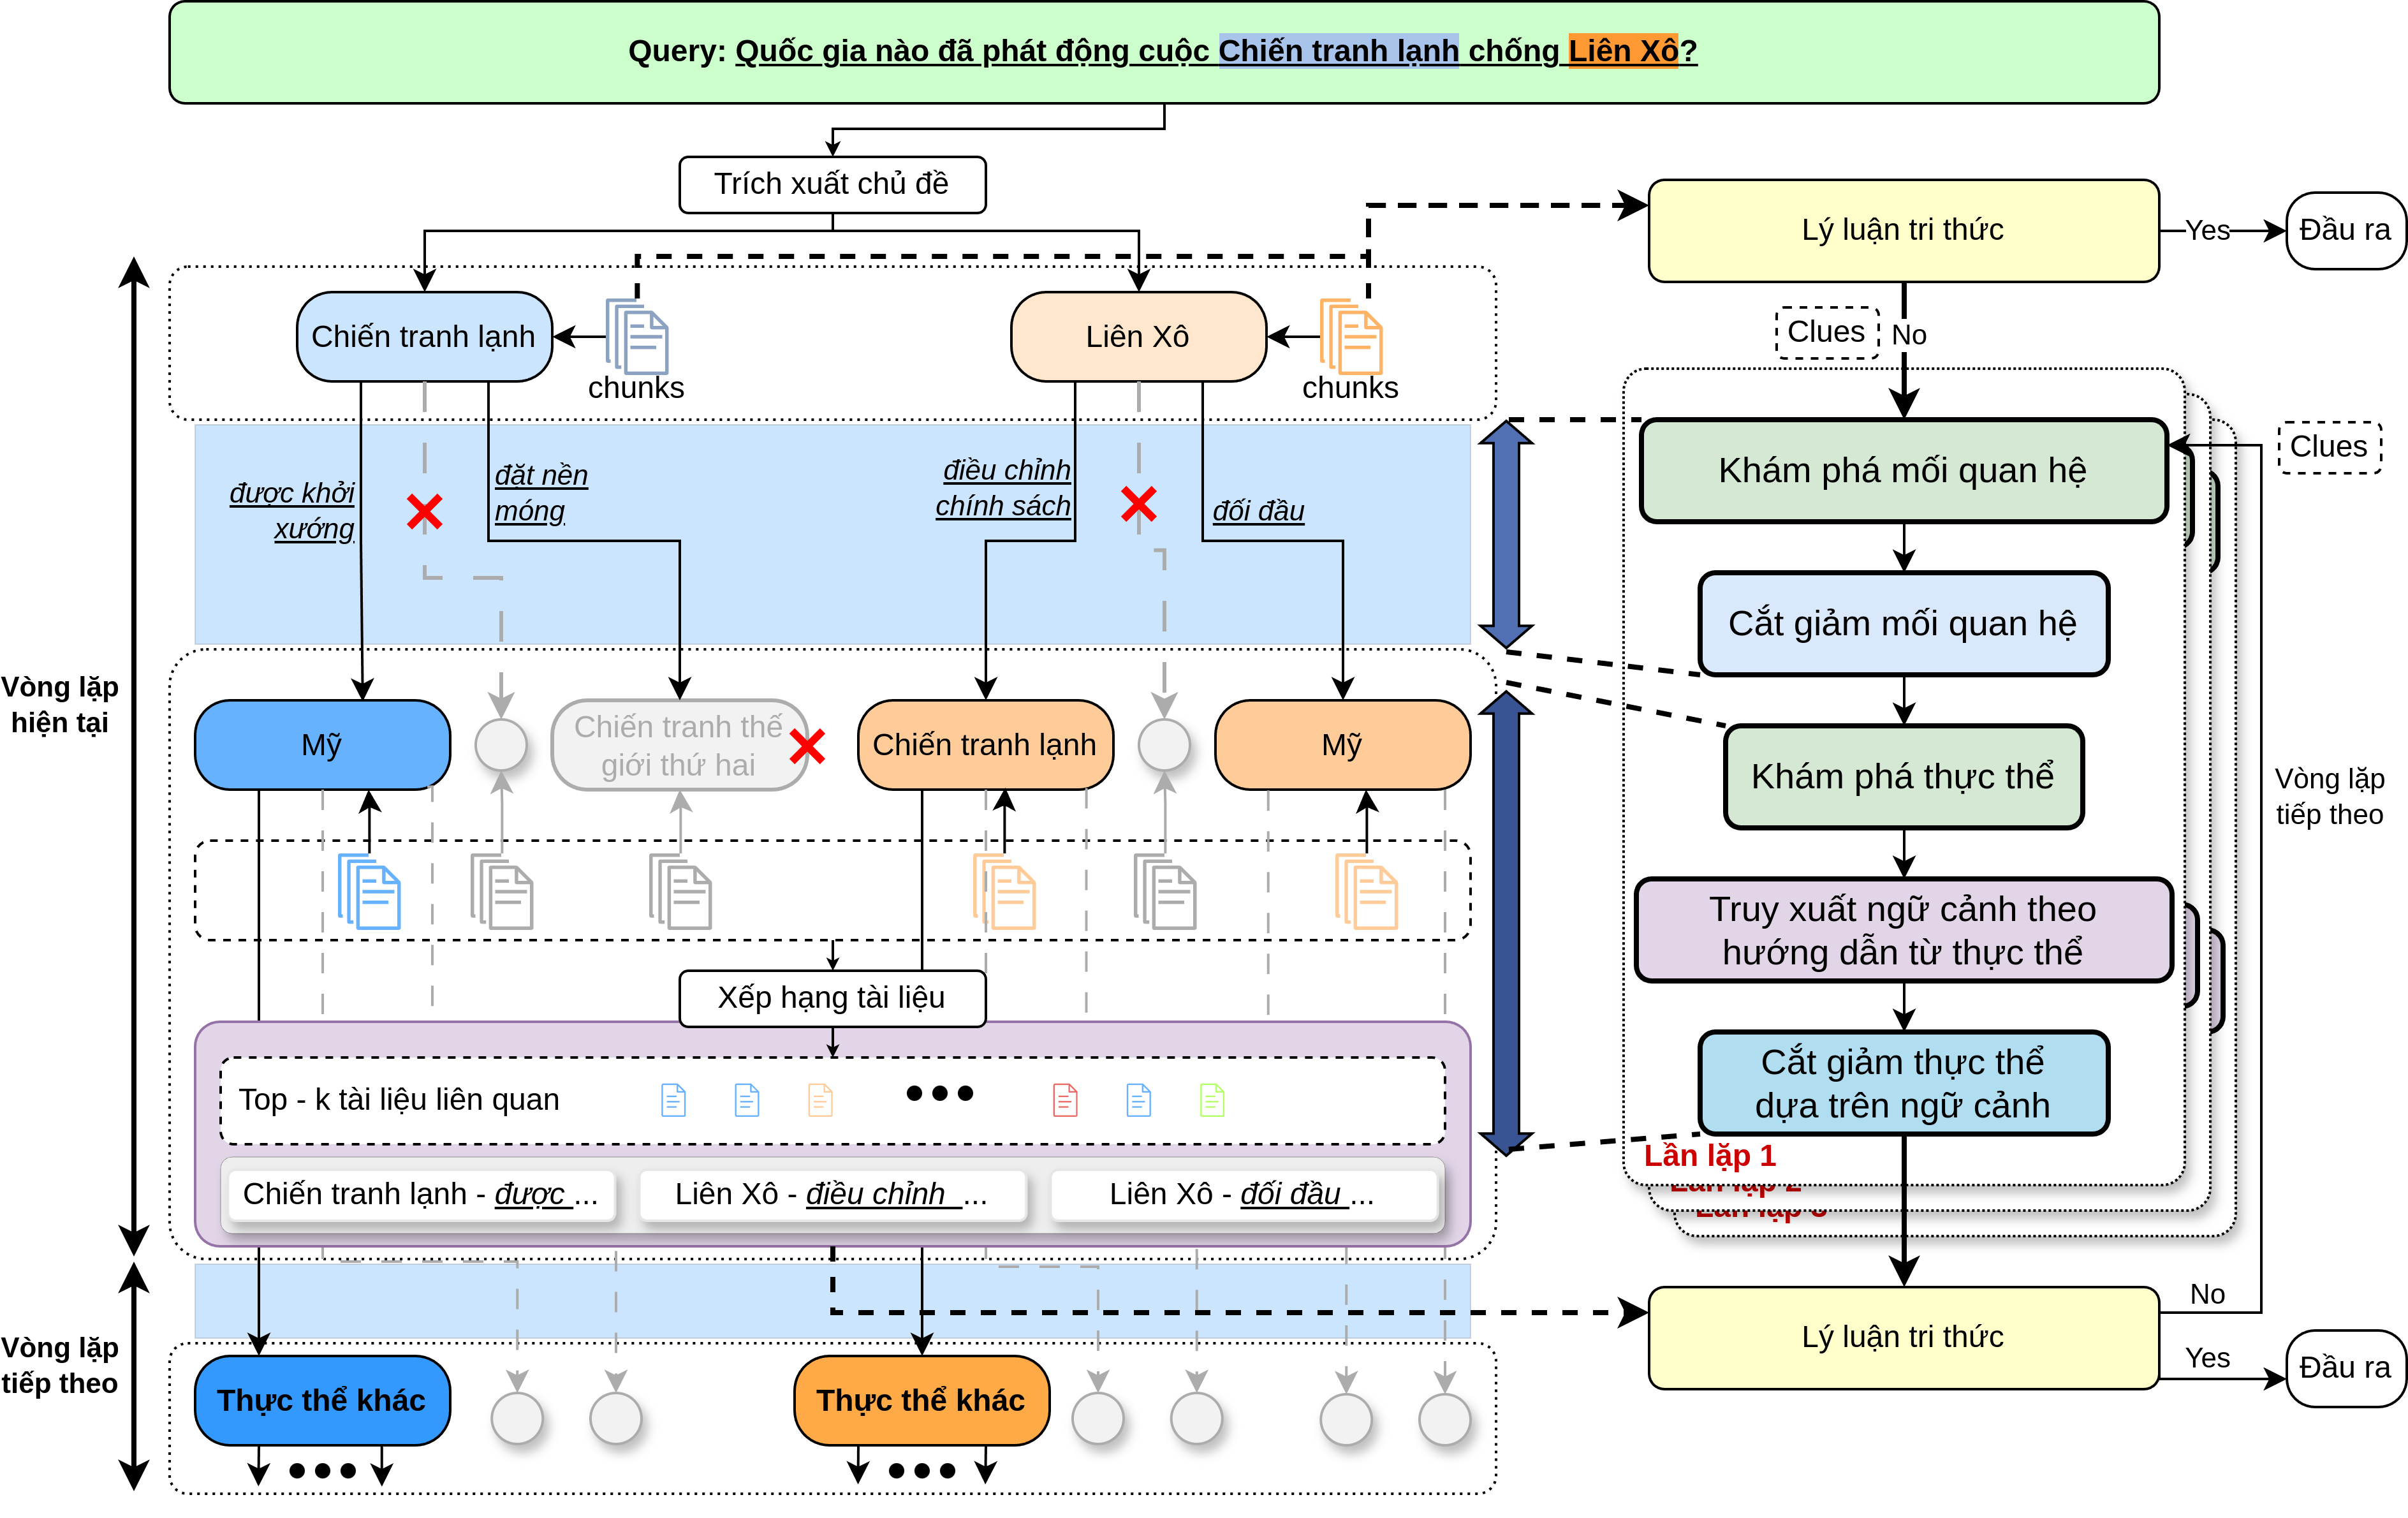
\includegraphics[width=1\textwidth]{Chapter3/Fig/pipeline.png}
    \caption{Mô hình \gls{rag} tích hợp truy xuất, suy luận đồ thị tri thức với truy xuất cơ sở dữ liệu vector}
    \label{fig:proposed_method}
\end{figure}


Phần này sẽ trình bày chi tiết từng bước của mô hình được đề xuất trong khóa luận này. Mô hình này sẽ bắt đầu với phần khởi tạo với nhiệm vụ trích xuất các thực thể từ câu hỏi đã cho làm các thực thể chủ đề ban đầu. Sau đó, nó thực hiện một quy trình lặp đi lặp lại việc khám phá tri thức và lý luận các tri thức được khám phá thông qua việc sử dụng LLM. Tại mỗi vòng lặp, bước “khám phá” sẽ truy xuất, tìm kiếm tri thức có chọn lọc bao gồm các quan hệ, thực thể liền kề với thực thể chủ đề hiện tại dựa trên \gls{kg} được xây dựng trong phần \ref{section:database_construction_method}, sử dụng các thực thể mới gặp phải để tinh chỉnh phạm vi truy xuất, từ đó nâng cao cả hiệu quả và độ chính xác. Rồi sau đó, sẽ xếp hạng và chọn lọc các thực thể dựa trên truy vấn và các ngữ cảnh thu thập được từ các tài liệu có liên quan để giảm thiểu sự mơ hồ từ đó tìm ra $top-N$ đường dẫn suy luận chứa thông tin liên quan nhất đến câu hỏi. Tiếp đến tại bước “lý luận”, sử dụng \gls{llm} đánh giá các thông tin, kiến thức có được từ các đường dẫn lập luận và ngữ cảnh dựa trên nó có đủ thông tin để trả lời câu hỏi. Quá trình này tiếp tục cho đến khi thu thập đủ thông tin thông qua $top-N$ đường lý luận để trả lời câu hỏi (được đánh giá bởi \gls{llm} trong bước "lý luận") hoặc đạt đến độ sâu tìm kiếm tối đa được định trước. Mô hình được mô tả chi tiết các bước thực hiện kèm theo ví dụ minh họa trong hình \ref{fig:proposed_method}.


\subsection{Khởi tạo}
\label{subsection:initialization}
Với đầu vào là câu hỏi $q$, bước đầu tiên là xác định thực thể xuất hiện trong q và liên kết chúng với các thực thể tương ứng trong đồ thị tri thức. Bước này có thể được hoàn thành dựa vào nhiều phương pháp liên kết thực thể (Entity Linking - EL) khác nhau, tiêu biểu có thể sử dụng \gls{llm}s hoặc các công cụ, mô hình chuyên về EL. Tiếp theo là bước đánh giá thực thể (Topic Evaluate - TE) để chọn ra những thực thể phù hợp nhất làm điểm bắt đầu cho việc khám phá trong một \gls{kg}. Bước này sẽ sử dụng \gls{llm} để đánh giá câu hỏi $q$ và các thực thể xuất hiện, từ đó chọn ra $N$ thực thể chủ đề $\mathcal{E_\text{topic}} (e_1, e_2, \dots, e_N)$ để làm điểm khởi đầu cho $n$ đường dẫn suy luận $\mathcal{P}(p_1, p_2, \dots, p_N)$. (Với $N$ là siêu tham số chiều rộng khám phá của mô hình hay số lượng đường dẫn suy luận tối đa được được giữ lại tại mỗi vòng lặp)


Trước khi bước vào lần đầu tiên truy xuất đồ thị, một mô hình \gls{drms} được sử dụng để chọn ra $top-k$ đoạn văn $Ctx^0$ từ các tài liệu liên kết với với các chủ đề ban đầu $\mathcal{E}_{\text{topic}}$. Sau đó \gls{llm} sẽ đánh giá thông tin này có đủ để trả lời câu hỏi hay không dựa vào kiến thức đã được huấn luyện của nó. Nếu \gls{llm} kết luận rằng thông tin hiện có đủ để trả lời câu hỏi, các bước tiếp theo là không cần thiết và có thể trực tiếp trả về câu hỏi cho người dùng. Ngược lại, nếu thông tin hiện có không đủ, mô hình sẽ sử dụng LLM với prompt \ref{tab:requery_prompt}  để dự đoán các manh mối, bằng chứng cần bổ sung để trả lời câu hỏi và tạo ra truy vấn phù hợp - $Clues$ - để lấy những thông tin hữu ích này.
\begin{equation}
    \centering
    Clues = Prompt_{\text{requery}}(q, Ctx^0)
    \label{eq:requery_prompt}
\end{equation}


\subsection{Khám phá tri thức}
\label{subsection:knowledge_exploration}
Phần này sẽ trình bày chi tiết cách mô hình được đề xuất lặp lại quy trình khám phá tri thức để thống nhất và gắn kết chặt chẽ các tri thức từ \gls{kg} và các đoạn văn được xây dựng trong phần \ref{section:database_construction_method}.


Tại thời điểm bắt đầu của vòng lặp thứ $I$, mỗi đường dẫn $p_n$ (với $n \in \{1, N\}$) bao gồm $I - 1$ bộ 3, một bộ ba ở đây tức là: $p_n = {\{(e_{s,n}^i, r_j^i, e_{o,n}^i)\}}_{i=1}^{I-1}$, trong đó $e_{s,n}^I$ và $e_{o,n}^I$ lần lượt biểu thị các thực thể chủ ngữ và thực thể tân ngữ, $r_j^I$ là một quan hệ cụ thể giữa chúng, các bộ ba $(e_{s,n}^I, r_j^I, e_{o,n}^I)$ và $(e_{s,n}^{I+1}, r_j^{I+1}, e_{o,n}^{I+1})$ được kết nối với nhau. Tập hợp các thực thể đuôi và các quan hệ trong $\mathcal{P}$ lần lượt được ký hiệu là $\mathcal{E}^{I-1} = {e_1^{I-1}, e_2^{I-1}, ..., e_n^{I-1}}$ và $\mathcal{R}^{I-1} = {r_1^{I-1}, r_2^{I-1}, ..., r_n^{I-1}}$. Quá trình lặp lại này gồm có 2 phần chính: nâng cao truy xuất đồ thị dựa trên ngữ cảnh và truy xuất ngữ cảnh thông qua hướng dẫn từ tri thức:


\subsubsection{Nâng cao truy xuất đồ thị thông qua ngữ cảnh:}
\label{subsubsection:graph_expansion}


Bằng cách tận dụng sự kết nối phong phú có cấu trúc của kiến thức trên đồ thị tri thức (KG), việc tìm kiếm trên đồ thị nhằm khám phá và thiết lập các khái niệm cấp cao cũng như mối quan hệ giữa câu hỏi và thông tin mục tiêu, vốn dường như cách xa nhau trong không gian ngữ nghĩa. Mô hình được đề xuất trong khóa luận bao gồm các bước sau đây.
\paragraph{Khám phá mối quan hệ (Relation Exploration):}
tại thời điểm bắt đầu của vòng lặp thứ $I$, mô hình sẽ tìm kiếm toàn bộ quan hệ được liên kết tới thực thể cuối cùng của mỗi reasoning path thông qua sử dụng hàm:
\begin{equation}
    \text{Edge}(e_j^{I-1}) = \{(r_{j, m}^{I}, h_m) | h_m \in \{True, False\}\}
    \label{eq:1}
\end{equation}
Hàm Edge() là hàm tìm kiếm các quan hệ (relationship) của thực thể. Trong đó $h$ biểu thị chiều của quan hệ $r_{j, m}^{I}$ đối với thực thể $e_j^{I-1}$.


\paragraph{Cắt giảm các quan hệ (Relation Prune):}
Thông qua phương trình \ref{eq:1} ta thu được các tập các mối quan hệ ứng viên
$\{{Edge(e^I_j )}\}^W_{j=1}$. Tại đây sẽ sử dụng phương pháp few-shot prompt để yêu cầu \gls{llm} đánh giá, lựa chọn và chấm điểm các mối quan hệ với các đường dẫn suy luận tương ứng có khả năng tìm thấy thực thể chứa thông tin ngữ cảnh phù hợp hữu ích cho việc giải quyết câu hỏi $q$. Rồi sau đó chọn ra $top-N$ mối quan hệ với các đường dẫn suy luận tương ứng có số điểm cao nhất để sử dụng cho bước tiếp theo. Tại đây, có 2 prompt được xây dựng để sử dụng:
\begin{equation}
    PROMPT_\emph{RP}(p_n , q, Edge(e^{I - 1}_n))
    \label{eq:2}
\end{equation}
và
\begin{equation}
    PROMPT_\emph{RP\_all} (q, {\{p_n, Edge(e^{I-1}_n)\}}^N_{n=1})
    \label{eq:3}
\end{equation}
Chi tiết của các prompt được trình bày tại phần phụ lục \ref{tab:relation_prune_prompt} và \ref{tab:relation_prune_prompt_all}. phương trình \ref{eq:2} được xây dựng với mục tiêu là gọi \gls{llm} nhiều lần cho việc cắt giảm mối quan hệ trên từng trên từng đường dẫn suy luận, trong khi đó phương trình \ref{eq:3} được xây dựng để xử lý việc chọn quan hệ phù hợp cho tất cả các reasoning paths trong 1 lần sử dụng LLM. Phương trình \ref{eq:2} đơn giản hóa nhiệm vụ của LLM và luôn giữ được các đường dẫn suy luận trước đó được tiếp tục, tuy nhiên nó lại thiếu hiệu quả khi phải sử dụng \gls{llm} nhiều lần và nhiều trường hợp giữ lại các đường dẫn không chứa thông tin hữu ích. Còn tại phương trình \ref{eq:3}, việc xử lý tất cả trong 1 lần giúp cho việc sử dụng \gls{llm} giảm đi từ đó nâng cao tốc độ suy luận và cho phép xem xét một cách tổng quan các mối liên kết giữa nhiều đường dẫn suy luận cùng lúc cùng lúc, tạo điều kiện cho việc đánh giá trở nên khách quan, chính xác hơn. Tuy nhiên, việc đưa toàn bộ các quan hệ với số lượng lớn đối với từng đấy các đường dẫn suy luận là một thách thức trong khả năng hiểu toàn bộ ngữ cảnh và đưa ra lựa chọn chính xác của \gls{llm}.


\paragraph{Khám phá thực thể (Entity Discovery):} Tại đây chúng ta có tập các đường dẫn suy luận với được chọn từ bước cắt giảm mối quan hệ với các mối quan hệ tương ứng được thêm vào. Cho một đường dẫn suy luận $p_n$ trong $\mathcal{P}$ với $e^{I - 1}_n$ là thực thể đuôi của $p_n$ và các mối quan hệ tương ứng $r^{I - 1}_n$. Tại đây mô hình sử dụng hàm sau:
\begin{equation}
    Tail(e^{I - 1}_n, (r^{I - 1}_n, h)) = \mathcal{C}^{I - 1}_n
    \label{eq:4}
\end{equation}
từ đó xác định được tập các thực thể ứng viên $\mathcal{C}^{I - 1}_n$ kết nốt với $e^{I - 1}_n$ thông qua quan hệ $(r^{I - 1}_n, h)$.




\subsubsection{Truy xuất ngữ cảnh thông qua hướng dẫn từ tri thức:}


Trong bước này, mô hình sẽ tập trung khai thác các thông tin hữu ích dựa theo các tri thức trích xuất được từ \gls{kg} thông qua phần \ref{subsubsection:graph_expansion}.


Sau khi xác định được tất cả các tập thực thể  ứng viên $\mathcal{C}^{I - 1}_n$ thông qua thực thi hàm \ref{eq:4}. Mô hình sẽ thu thập các tài liệu được liên kết với các thực thể ứng viên, rồi kết hợp với $top-k$ tài liệu $Ctx^{I - 1}$ để đánh giá, xếp hạng những tài liệu và chọn ra $top-k$ tài liệu có điểm cao nhất. Say đây là các bước chi tiết thực hiện:
\paragraph{Truy xuất ngữ cảnh, đoạn văn dựa trên các thực thể:}
để tìm kiếm những thông tin hữu dụng từ trong các tài liệu ngữ cảnh liên kết với các thực thể ứng viên, mô hình sẽ sử dụng \gls{drms} để tính điểm liên quan của các tài liệu. Thay vì tính toán trực tiếp điểm liên quan giữa tài liệu ngữ cảnh và câu hỏi (từ đó bỏ qua ngữ cảnh giữa tài liệu và thực thể tương ứng của nó) điểm sẽ được tính thông qua việc chuyển đổi các đường dẫn suy luận $p_n$ tương ứng với từng $\mathcal{C}^{I - 1}_n$  thành một câu ngắn gọn và thêm nó vào ngữ cảnh rồi từ đó sẽ sử dụng mô hình \gls{drms} để đánh giá điểm liên quan giữa ngữ cảnh mới này và câu hỏi. Đây là phương trình tính điểm liên quan giữa tài liệu thứ $z$ của thực thể ứng viên $chunk^{I-1}_{n,z}$ như sau:
\begin{equation}
    srl(chunk^{I-1}_{n,z}) = \text{DRM}(q, [brief\hspace{-0.1cm}\_sentence(p_n), :chunk^{I-1}_{n,z}])
    \label{eq:5}
\end{equation}
Vì các tài liệu được lưu trữ dưới dạng cây tài liệu, nên giữa các tài liệu luôn có mối quan hệ về ngữ cảnh, vậy nên để điểm của mỗi tài liệu sẽ chịu tác động từ các tài liệu khác. Hiện tại chưa có nghiên cứu nào về cách tính sự tương tác giữa các tài liệu. Vậy nên sau nhiều lần thực nghiệm, tôi đã xây dựng phương trình tính toán sự liên quan giữa tài liệu $u$ và tài liệu $v$ trong việc trả lời câu hỏi $q$ dựa trên kết quả của phương trình \ref{eq:5} như sau (với $\alpha$ là một siêu tham số để điều chỉnh mức độ tương tác giữa các tài liệu):
\begin{equation}
    interaction(u,v) = \dfrac{1}{Distance(u, v)^2 + \alpha} \times srl(u) \times srl(v)
    \label{eq:6}
\end{equation}
Điểm cuối cùng của mỗi tài liệu sẽ là trung bình cộng của điểm liên quan giữa tài liệu đó với tất cả các tài liệu có liên kết với chúng cộng với điểm phương trình \ref{eq:5} của chúng:
\begin{equation}
    \begin{split}
        c\_score^{I-1}_{j,z} = \dfrac{1}{|linked\_chunks|}\times \sum_{v \in linked\_chunks} interaction(chunk^{I-1}_{n,z}, v) \\
        +   srl(chunk^{I-1}_{n,z})
    \end{split}
    \label{eq:7}
\end{equation}
trong đó $linked\_chunks$ là tập hợp các tài liệu liên kết với $chunk^{I-1}_{n,z}$. Sau đó dựa trên điểm, mô hình sẽ chọn ra $top-k$ tài liệu
\begin{equation}
    \centering
    Ctx^I = \{ chunk_i \mid i \in \arg\max_{i_1, i_2, \dots, i_k} \left( Chunk_\text{related}^I \right) \} ,
\end{equation}


với $Chunk_\text{related}^I$ là toàn bộ điểm của tất cả các tài liệu liên kết với các thực thể ứng viên $\mathcal{C}^{I - 1}_n$ để sử dụng cho bước tiếp theo.
\paragraph{Cắt giảm thực thể (Entity Prune):}


Dựa vào $Ctx^I$ được chọn ra từ bước truy xuất ngữ cảnh, mô hình sẽ sử dụng mô hình \gls{llm} để đánh giá chấm điểm các đường dẫn suy luận với đuôi là các thực thể ứng viên tương ứng để chọn ra những đường dẫn suy luận có khả năng trả lời câu hỏi tốt nhất và để sử dụng cho các vòng lặp tiếp theo. Dưới đây là prompt được sử dụng cho việc cắt giảm thực thể:
\begin{equation}
    PROMPT_\emph{EP}(Ctx^I, q, p_n, \mathcal{C}^{I - 1}_n)
    \label{eq:8}
\end{equation}
Sau đó sẽ chọn ra $top-N$ đường dẫn suy luận tốt nhất để sử dụng cho vòng lặp kế tiếp. Chi tiết về prompt được trình bày tại phần phụ lục \ref{tab:entity_prune_prompt}.


\subsection{Suy luận từ tri thức kết hợp}
\label{subsection:integrated_reasoning_from_knowledge}
Cuối vòng lặp thứ $i$, mô hình sẽ sử dụng \gls{llm} với toàn bộ tri thức tìm được từ các bước phía trên, bao gồm các đường dẫn suy luận, manh mối $Clue^{I-1}$ và $Ctx^I$ để đánh giá liệu rằng các thông tin đó có đủ để trả lời câu hỏi, với $Clue^{I-1}$ là phản hồi truy xuất từ lần lặp phía trước với mục tiêu là để duy trì tri thức hữu ích từ bối cảnh lịch sử. Nếu \gls{llm} đánh giá rằng kiến thức được cung cấp là đủ để đưa ra câu trả lời, sẽ trực tiếp trả về câu trả lời. Ngược lại, thì sẽ tạo ra truy vấn $Clue^{I}$ và bắt đầu vòng lặp tiếp theo. Để hướng dẫn \gls{llm} đánh giá, mô hình sẽ sử dụng prompt sau:
\begin{equation}
    PROMPT_\emph{RS}(q, \mathcal{P}, Clue^{I-1}, Ctx^I) =
    \begin{cases}
        \text{Ans.}, & \text{(Có)}    \\
        Clues^i,     & \text{(Không)}
    \end{cases}
    \label{eq:9}
\end{equation}
Chi tiết về prompt sẽ được trình bày tại phần phụ lục \ref{tab:reasoning_prompt}.
